\section{Aufbau einer spezifischen View als Vertreter}
Die Datei \texttt{SinglePlantView.vue} bildet das Grundgerüst für die Detailansicht einer einzelnen Pflanze in. Diese View ist modular aufgebaut und umfasst mehrere miteinander koordinierte Komponenten, die sowohl funktional als auch visuell klar voneinander getrennt sind. Die Umsetzung folgt modernen Prinzipien komponentenbasierter Architektur in Vue, wobei jede logische Funktionseinheit in eine eigene Komponente oder ein strukturell abgegrenztes Template-Element eingebettet ist. Die Aufteilung in Subbereiche ergibt sich direkt aus den Bedürfnissen einer klaren Benutzerführung sowie der funktionalen Entkopplung von Darstellung und Logik. Eine Darstellung der kompletten Komponente ist in \vref{fig:SingelPlantView} zu sehen.

\begin{figure}[H]
	\centering
	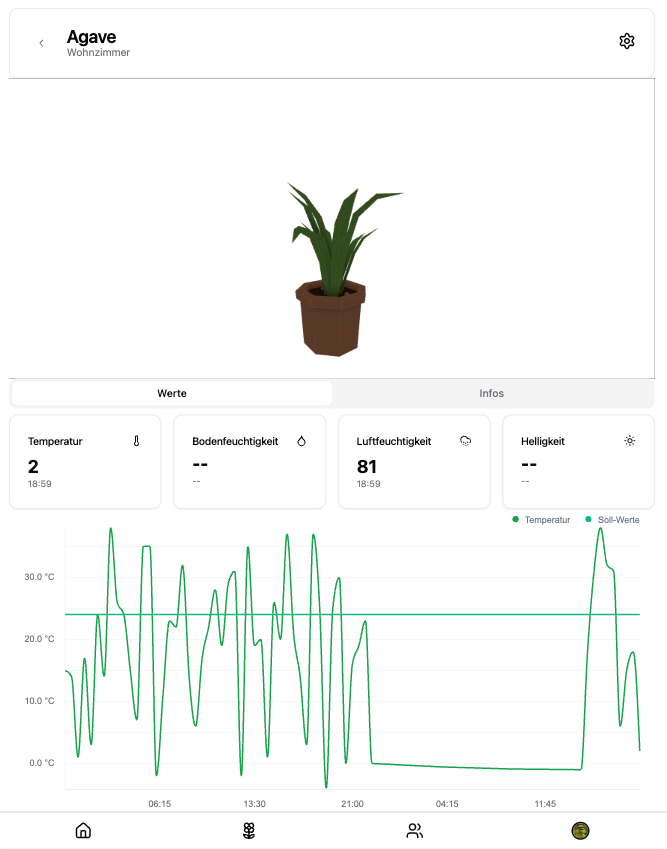
\includegraphics[scale=.5]{"./Umsetzung/images/sensora.png"}
	\caption{SinglePlantView in Aktion}
	\label{fig:SingelPlantView}
\end{figure}

Im oberen Abschnitt ist die Komponente \texttt{NavCard.vue} zu finden. Die ist für Überschriften mit einfacher Navigation zuständig in mehreren Views. Dieser Bereich ist durch die statische Anzeige des Pflanzennamens („Agave“) sowie der Rauminformation („Wohnzimmer“) gekennzeichnet. Diese Informationen werden direkt aus dem zentralen Datenmodell geladen, welches über ein Pinia-Store-Modul eingebunden ist. Der Benutzer erhält hier sofort kontextuelle Informationen zur Zuordnung der Pflanze im System.

Unmittelbar darunter befindet sich die 3D-Visualisierung der Pflanze, welche als zentrales visuelles Element prominent dargestellt ist. Diese Visualisierung basiert auf einem in der Datei \texttt{plantAvatars.ts} definierten Pflanzenmodell, das auf Basis des Pflanzentyps dynamisch geladen wird. Die Komponente zur Darstellung selbst ist als \texttt{<plant3d />} eingebettet, wobei ein Canvas-Rendering mit \texttt{Three.js} verwendet wird. Die visuelle Präsentation trägt zur Gamification der Anwendung bei, indem sie die emotionale Bindung und Wiedererkennung der Pflanzen fördern soll \cite{Werbach2012}.

Darunter folgt ein horizontal geteilter Abschnitt mit zwei Tabs: „Werte“ und „Infos“. Der Reiter „Werte“ ist standardmäßig aktiv, was sich in der visuellen Hervorhebung des Tabs zeigt. Innerhalb dieses Tabs sind vier Kartenkomponenten (Card-Komponenten) zu erkennen, die jeweils einen Umweltsensorwert repräsentieren: Temperatur, Bodenfeuchtigkeit, Luftfeuchtigkeit und Helligkeit. Diese sind als wiederverwendbare UI-Komponenten realisiert, die dynamisch Daten einlesen und anzeigen. Die Temperatur- und Luftfeuchtigkeitswerte sind im dargestellten Beispiel verfügbar („18 °C“ und „70 \%“), während Bodenfeuchte und Lichtstärke als nicht verfügbar („--“) markiert sind – ein Hinweis auf fehlerhafte oder fehlende Sensoranbindung. Jede Karte zeigt zusätzlich den letzten Messzeitpunkt, was eine präzise Einordnung der Datenqualität ermöglicht.

Der untere Teil der View wird durch die Verlaufsgraphen-Komponente dominiert, die in \texttt{PlantMeasuredValuesChart.vue} ausgelagert ist. Diese Komponente nutzt den Wrapper von \texttt{shadcn-vue} für \texttt{unovis}, um Messwerte über einen Zeitraum hinweg grafisch darzustellen. Im dargestellten Screenshot ist ein Temperaturliniendiagramm zu sehen, das über 24 Stunden  Werte anzeigt. Ein horizontaler Zielwert (Soll-Wert) ist ebenfalls dargestellt, was dem Benutzer eine sofortige Einschätzung der Umweltbedingungen erlaubt. Die Auswahl dieses Visualisierungsformats folgt dem Prinzip der kognitiven Entlastung: Durch einfache visuelle Kodierung können Zustände schneller interpretiert werden als durch numerische Tabellen.

Abgeschlossen wird die Komponente durch die \texttt{BottomNavBar.vue}, die über vier Icons eine einfache Navigation innerhalb der Anwendung ermöglicht. Diese sind als feste UI-Komponenten realisiert, wobei ein Button speziell dem Rücksprung zur Pflanzenübersicht oder der Startseite dient.

Insgesamt ergibt sich aus dieser strukturierten Aufteilung ein konsistentes, nutzerzentriertes Interface, das sowohl eine einfache Übersicht als auch eine tiefgehende Analyse einzelner Pflanzendaten erlaubt. Die klare funktionale Trennung – Datenanzeige oben, Visualisierung unten, Navigation ganz unten – folgt bewährten Usability-Prinzipien, die sich in wissenschaftlicher Literatur zur Mensch-Computer-Interaktion vielfach bewährt haben \cite{norman2013design}.


